\newthought{Counting words with constraints} is the topic of the problem\ in this note. This problem was posed by a coworker at a lunch discussion.

\begin{marginfigure}[0.01in]

\includegraphics[scale=0.5]{cards.pdf}
\end{marginfigure}

\vspace{10 mm}
\begin{problem}
When you go see the Penn \& Teller Magic Show in Las Vegas you can get a random card from the \textbf{Perfectly Ordinary Deck of Cards} at the entrance. How many times do you have to see the show to collect the full deck.
\end{problem}

We assume the supply of cards at the entrance is endless and thoroughly shuffled. This allows us to work with a probability model of drawing with replacement where each card is equally likely to be drawn with probability $\frac{1}{52}$. At each visit we draw a card\footnote{You can get two cards at each visit to the show in Las Vegas. Drawing only one card is a simplification to keep the expressions smaller. The case with two cards is similar but the expressions get a little bigger because you have more cases of the card sequence right before the visit that achieves full deck. We will point out the differences at the end of this note.}.
After $k$ visits we have built up a sequence of cards which we model as a word $w_k=(c_1, c_2, \ldots, c_k)$ of size $k$ from an alphabet of size $52$ ($\forall c_i: c_i \in \{1, \ldots, 52\}$). Our random variable $X$ is the number of visits needed to achieve a full deck. The probability $P(X=k)$ means that it took $k$ visits to achieve the full deck. 

The key observation is this: if it took $k$ visits to achieve full deck then at visit $k-1$ the corresponding word of cards $w_{k-1}=(c_1, c_2, \ldots, c_{k-1})$ is missing just one card and all the other cards appear at least once in the word\footnote{It might be easier to see this with a concrete card. Imagine you are drawing an ace of spades at visit $k$ and getting the full deck. This means that before the visit $k$ you are still missing the ace of spades. If not, then drawing the ace of spades at visit $k$ wouldn't complete the deck. Getting the full deck at visit $k$ also means that you are not missing any other cards before the visit $k$, otherwise if one of the other cards would be missing then drawing an ace of spades again wouldn't complete the deck.}.

Let $\mathcal{A} = \{1, 2, \ldots, 52\}$ be our alphabet and $L_k(\mathcal{A}) = \{(c_1, c_2, \ldots, c_k): \forall i: 1 \leq i \leq k: c_i \in \mathcal{A}\}$ the set of all the words of length $k$ with letters (cards) from the alphabet $\mathcal{A}$. Let $M_k(c)$ be the set of words of length $k$ where letter $c$ does not occur in the word and every other letter occurs at least once:

\begin{align*}
M_k(c) = \{(c_1, c_2, \ldots, c_k): &(\forall i: 1 \leq i \leq k: c_i \in \mathcal{A} \wedge c_i \neq c) \wedge \\
& (\forall d \in \mathcal{A} \setminus \{c\}: \exists i: 1 \leq i \leq k: c_i = d)\}
\end{align*}

So now let us assume that at visit $k$ we draw letter $c$ and get the full deck. From our previous argument above we know that then the word $w_{k-1}$ we built in the previous $k-1$ visits has to be in $M_{k-1}(c)$.


The probability that at visit $k$ we draw letter $c$ and get the full deck is thus the probability of drawing card $c$ times the probability that $w_{k-1} \in M_{k-1}(c)$. It follows that:

$$
P(X=k) = \sum_{c \in \mathcal{A}} \frac{1}{|\mathcal{A}|} \frac{|M_{k-1}(c)|}{|L_{k-1}(\mathcal{A})|}
$$

As we will see below, $|M_{k-1}(c)|$ is the same for all cards $c$, so for some fixed card $c_0$ we have $\forall c \in \mathcal{A}: |M_{k-1}(c)| = |M_{k-1}(c_0)|$. Then

$$
P(X=k) = \frac{|M_{k-1}(c_0)|}{|L_{k-1}(\mathcal{A})|} \sum_{c \in \mathcal{A}} \frac{1}{|\mathcal{A}|} = \frac{|M_{k-1}(c_0)|}{|L_{k-1}(\mathcal{A})|}
$$

We already know that 

$$
|L_{k-1}(\mathcal{A})| = |\mathcal{A}|^{k-1}
$$

What is left to do to compute $P(X=k)$ is count $|M_{k-1}(c_0)|$. To avoid carrying around the $k-1$ we will count $|M_k(c_0)|$ instead and adjust afterwards.

How do we compute $|M_k(c_0)|$ ? We have two constraints on the words in $w_k=(c_1, c_2, \ldots, c_k) \in M_k(c_0)$:

\begin{align*}
\text{constraint } C_1 &: \forall i: 1 \leq i \leq k: c_i \in \mathcal{A} \wedge c_i \neq c_0 \\
\text{constraint } C_2 &: \forall d \in \mathcal{A} \setminus \{c_0\}: \exists i: 1 \leq i \leq k: c_i = d
\end{align*}

Constraint $C_1$ is easy to satisfy: we just use the alphabet without letter $c_0$: $\mathcal{A}_1 = \mathcal{A} \setminus \{c_0\}$.

For constraint $C_2$ we could try to eliminate all the subsets of $L_{k}(\mathcal{A}_1)$ with words missing one letter from $\mathcal{A}_1$, all the subsets with words missing two letters from $\mathcal{A}_1$ and so on all the way to subsets with words missing all but one letter from $\mathcal{A}_1$. Something like this:

$$
|M_k(c_0)| = |L_k(\mathcal{A}_1)| - \sum_{\mathcal{B} \subset \mathcal{A}_1} |L_k(\mathcal{A}_1 \setminus \mathcal{B})|
$$

\newpage

But we have to be careful here. The subsets that we aim to eliminate are not disjoint and this would lead to overcounting\footnote{Subsets with two missing letters are also subsets with one missing letter. Subsets with three missing letters are also subsets with two missing letters and subsets with one missing letter. And so on. It is indeed a use case for the inclusion-exclusion principle in combinatorics: \\ \bibentry{wikiInclusionExclusionPrinciple}.}. So instead the correct way to count this is:

$$
|M_k(c_0)| = \sum_{i = 0}^{|\mathcal{A}_1| - 1} (-1)^i \sum_{\mathcal{B} \subset \mathcal{A}_1, |\mathcal{B}|=i} |L_k(\mathcal{A}_1 \setminus \mathcal{B})|
$$

There are $\binom{|\mathcal{A}_1|}{i}$ subsets $\mathcal{B}$ of size $i$ and for each $|L_k(\mathcal{A}_1 \setminus \mathcal{B})| = (|\mathcal{A}_1| - i)^k$. It follows that

$$
|M_k(c_0)| = \sum_{i = 0}^{|\mathcal{A}_1| - 1} (-1)^i \binom{|\mathcal{A}_1|}{i} (|\mathcal{A}_1| - i)^k
$$

We have all the pieces now. We can adjust back to $k-1$ and also use $|\mathcal{A}|=52$ to make a nice, closed formula for $P(X=k)$:

$$
P(X=k) = \frac{1}{52^{k-1}} \sum_{i = 0}^{50} (-1)^i \binom{51}{i} (51 - i)^{k-1}
$$

Plugging this into \href{https://www.wolframcloud.com/obj/75d50b79-164a-4bed-a4b5-7592d2488169}{Mathematica} we can see the distribution and the cumulative distribution:\\


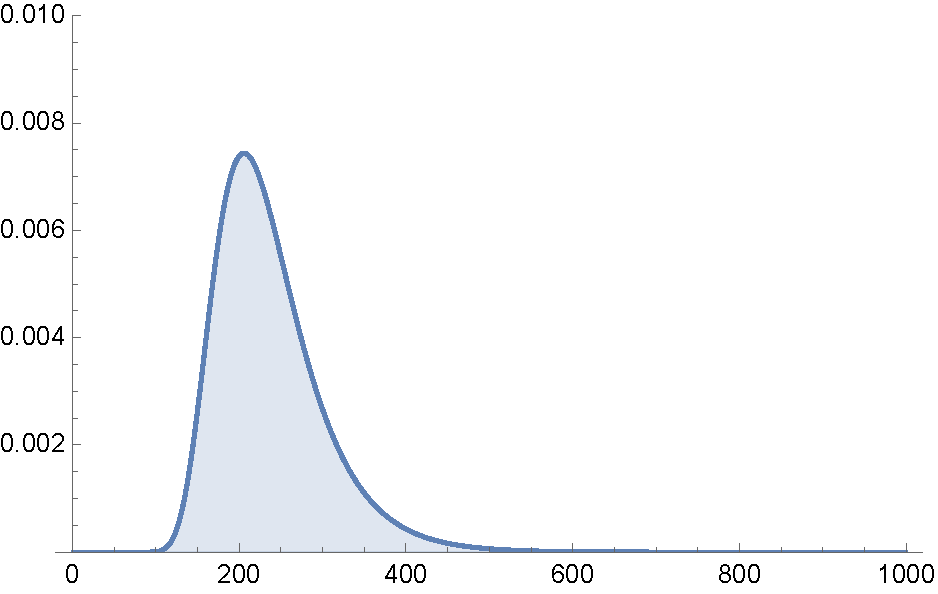
\includegraphics[scale=0.7]{probs.pdf}

 
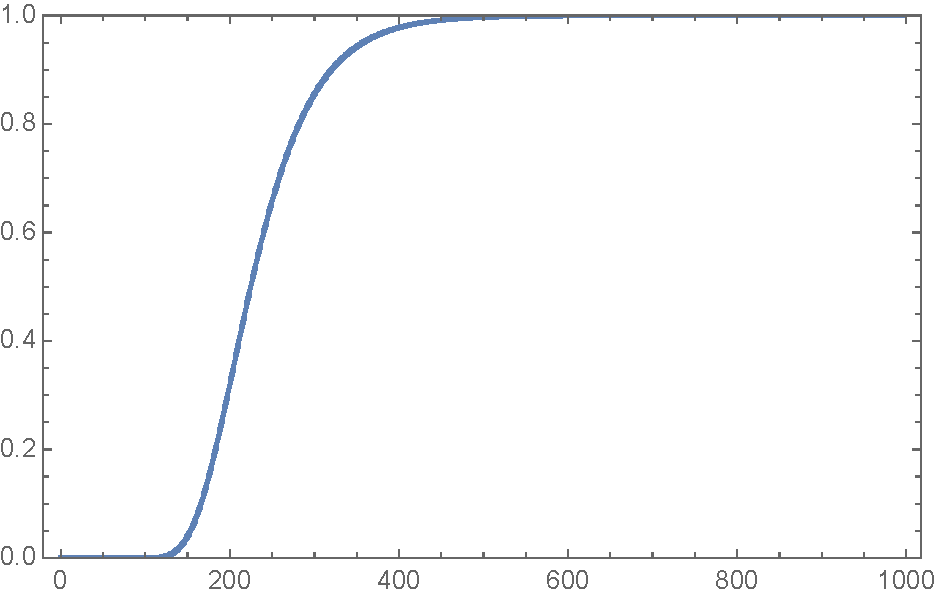
\includegraphics[scale=0.7]{cumulative.pdf}


It looks like around 400 visits will most likely get you a full deck. It might be cheaper to buy the full deck from the \textbf{Penn \& Teller} online store.

\newpage

It is always a good idea to double-check our result with a simulation\footnote{This is how I discovered a bug in my initial calculation. The listing is from my coworker that suggested the problem.}. The Python program below runs trials and records the number of visits necessary for a full deck:

\lstinputlisting[language=Python, basicstyle=\small, frame=trBL, caption={Simulation}]{simulation.py}

The results confirm that at least we are not orders of magnitude off: 
\begin{lstlisting}
n=100000
p0:   95
p25:  190
p50:  225
p75:  269
p100: 822
\end{lstlisting}

As promised, what are the differences when two cards are drawn at each visit. The constraints on the words right before the visit that achieves full deck are a little bit more complicated: there could be one or two cards missing. When one card is missing, the missing card could come in once or twice on the last visit. That's more or less it. Working out a closed formula for this is left as an exercise to the reader.
